\documentclass[journal ]{new-aiaa}
\usepackage[utf8]{inputenc}
\usepackage{textcomp}
\usepackage{subcaption}
\usepackage{float}


\usepackage{graphicx}
\usepackage{amsmath}
\usepackage[version=4]{mhchem}
\usepackage{siunitx}
\usepackage{longtable,tabularx}
\setlength\LTleft{0pt} 

\newcounter{ctab}
\setcounter{ctab}{1}

\title{Propeller Optimization at Different Blade Counts}

\author{Joseph Spencer \footnote{Undergraduate Researcher, Brigham Young University FLOW Lab.}}
\affil{Brigham Young University, Provo, Utah, 84601} 

\begin{document}

\maketitle

\begin{abstract}

propellers can be modified to perform better under a variety of conditions. One project completed as part of my research for the Brigham Young University FLOW Lab explores ideal design variables for propeller performance. This investigation used computer simulations to find the optimal chord length magnification and the optimal pitching angle for a propellor's efficiency. This report defines the operating conditions used in this optimization, presents propellors that were optimized at several blade counts, and discusses areas of possible future development in this research. I found that for the operating conditions used, propellors with the chord reduced to the optimization's lower limit, 50 percent, with negative pitching angles were the most efficient. These results could be applied to propellors designed to produce the maximum output power for a given input power requirement, without regard to other desired outputs. Future work could combine these findings with other conditions to find the most efficient propellor that can also provide a required amount of thrust or operate at a variety of different rotational velocities.

\end{abstract}


\section{Introduction}

\lettrine{P}{ropellors} come in a variety of different shapes and sizes. This paper describes how I used one propeller, an APC 10x7 rotor\footnote{Rotor geometry obtained from the UIUC database at \url{https://m-selig.ae.illinois.edu/props/volume-1/propDB-volume-1.html}} with a NACA 4412 airfoil\footnote{propeller geometry obtained from supporting information for CCBlade.jl at \url{https://github.com/byuflowlab/CCBlade.jl/tree/master/data}}, as a baseline to optimize a propeller's efficiency at a specific advance ratio. Because different blade counts could be more appropriate for different applications, I optimize and compare blade counts of 2, 3, and 4 in this report. I also compares the optimized propellors of each different blade count.

Computer simulations are very useful for modeling propellers. It would require significant investment of time, space, and money to perform an optimization like this by physically propellers. In the simulation used in this report, I instead computationally compared the properties of hundreds of slightly different propellers to obtain a final result. The first potential-flow codes, programs for modeling the pressure distribution of rotors, were developed in the 1960s and 1970s. Xfoil, a program used to create the airfoil model used in this project, was first developed by MIT in the 1980s, with its current version dating to 2013. Xfoil.jl was developed by Taylor McDonnell.\footnote{More information about both Xfoil and Xfoil.jl is available at \url{https://flow.byu.edu/Xfoil.jl/stable/} and \url{https://en.wikipedia.org/wiki/XFOIL}}

This paper first reviews the procedure I used in the rotor optimization, including the objective function used in the optimization and the initial conditions and constraints applied. Next, I review the results and compare them with each other. Finally, I draw conclusions based on the results of this optimization and discusses their meaning. All code used for each section of this report can also be accessed through a GitHub repository.\footnote{This repository can be accessed in the Rotor-Design branch of \url{https://github.com/JoeSpencer1/497R-Projects/tree/Final-Report}}


\section{Methods}

Computational stimulations of propellers allow researchers to perform low-risk studies and develop designs more quickly. I performed this project using Julia programming language.\footnote{Julia is available at \url{https://julialang.org}.} Jula is available for free and is useful for a variety of reasons. Like other languages, it can easily store data in vectors and perform rapid calculations with these objects. It is compiled just-in-time with precompiled functions, which makes it run faster than interpreted languages like python without needing to be totally compiled before running like C\footnote{This article describes some of the benefits of Julia. \url{https://towardsdatascience.com/5-ways-julia-is-better-than-python-334cc66d64ae}}. Julia  packages, including those used during this semester, are also easily available from a package manager.

\subsection{Models}

Some Julia packages used for this project include Xfoil.jl,\footnote{Xfoil.jl is available at \url{https://github.com/byuflowlab/Xfoil.jl}} CCBlade,jl,\footnote{CCBlade.jl is available at \url{https://github.com/byuflowlab/CCBlade.jl}} and SNOW.jl.\footnote{SNOW.jl is available at \url{https://github.com/byuflowlab/SNOWl.jl}} Xfoil.jl analyzes the lift, drag, and moment coefficients of an airfoil from its geometry and angle of attack using a potential-flow code with a panel method. This divides the airfoil into many small surfaces and finds the lift, drag, and moment forces at each of the smaller surfaces. 

CCBlade.jl uses blade element momentum (BEM) theory.\footnote{More information about BEM theory can be found at \url{https://en.wikipedia.org/wiki/Blade_element_momentum_theory}} BEM theory, which combines blade element theory and momentum theory, calculates the axial and tangential induction factors and the twist angle, the angle between the free stream velocity and the tangential velocity of the propeller. After these three quantities are found, they are combined to find forces acting in all directions on the propeller\cite{CCBlade}.

The propeller in this design was created beforehand and included in the documentation for CCBlade.\footnote{Same address listed in introduction note, \url{https://github.com/byuflowlab/CCBlade.jl/tree/master/data}} Airfoil data could be created using XFoil.jl, but I selected this data because its domain had already been widened using Viterna extrapolation to include a complete range of angles of attack\footnote{Further explanation of this method is available at \url{https://flow.byu.edu/CCBlade.jl/stable/howto/}}. The airfoil polars used to analyze this are presented in the following figure. 

\begin{figure}[H]
\centering
 	\subfloat[lift coefficient]{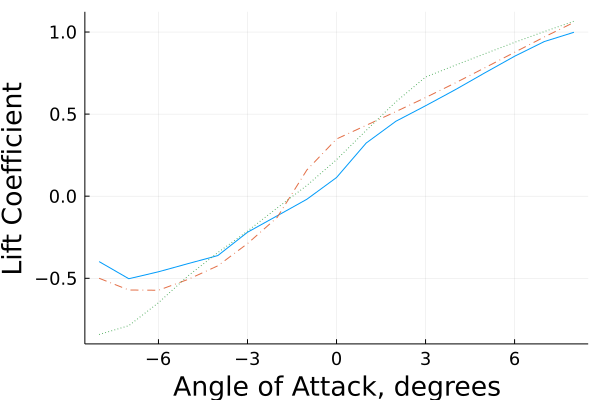
\includegraphics[width = .35\textwidth]{Plots/Figure13.png}}
	\subfloat[drag coefficient]{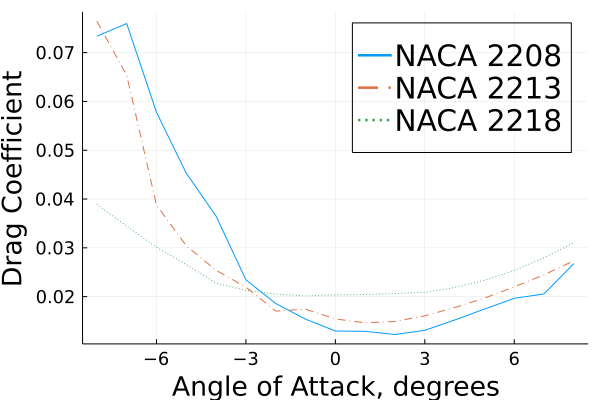
\includegraphics[width = .35\textwidth]{Plots/Figure14.png}}
	\caption{Lift and drag experienced by NACA 4412 airfoils}
	\captionsetup{aboveskip=0pt,font=it}
	\caption*{These plots show how lift and drag change for an airfoil at different angles of attack.}
	\label{afplot}
\end{figure}

I then placed the airfoil on the APC 10x7 rotor used in the project, and evaluated its torque and power coefficients across a range of advance ratios with CCBlade.jl. Propellers in the optimization were compared at a specific advance ratio, $J=0.472$, which is listed and explained later in this report in the bottom entry of table \ref{ctab}. I found the propeller's total torque and total moment from the torque output of the propeller's CCBlade.jl evaluation and from integrating the normal and tangential stresses.

\subsection{Optimization}

Once I found the propeller's initial torque and moment at this advance ratio, I multiplied them by a safety factor of $n=1.1$. This safety factor provided maximum limits for the propeller torque and moment to ensure that the SNOW.jl optimization would find the most efficient propeller that still had reasonable input torque and power requirements to be run by the same motor and made of the same materials as the initial propeller.

In addition to restrictions on the moment and torque mentioned previously, the cord thickness was kept within a factor of 2 of the original and the pitching angle was kept between $-90^{\circ}$ and $90^{\circ}$. These constraints are listed in equation \ref{optimization} after the torque and moment constraints. They ensured that the optimization found a reasonable solution confined to realistic limits.

In this optimization, I modified the chord length and pitching angle to find the most efficient propeller. The optimization is shown in equation \ref{optimization}. 

\begin{equation}
	\begin{aligned}
		\mathrm{maximize:}& ~~ \eta \\
		\mathrm{with~respect~to:}& ~~ c & \multicolumn{1}{l}{$\theta$} \\
		\mathrm{subject~to:}& ~~ 50\% \leq c \leq 200\% & -90^{\circ} \leq \theta \leq 90^{\circ} \\
		& M_{n} \leq 1.1 \times M_{n0} & M_{t} \leq 1.1 \times M_{t0} \\
		& T \leq 1.1 \times T_{0} \\
	\end{aligned}
	\label{optimization}
\end{equation}

Table \ref{ctab} shows shared features of each of the propellers optimized. The advance ratio, $J$, is available from other variables already listed in the table by equation \ref{Jequations}, in which $v_{\infty}$ is the free stream velocity, $n$ is the rotational velocity in revolutions per second, and $D$ is the outer diameter.

\begin{equation}
	\begin{aligned}
	J = \frac{v_{\infty}}{n D} \\
	J = \frac{12}{(\frac{6000}{60}) 0.254}
	\end{aligned}
	\label{Jequations}
\end{equation}

\begin{table}[H]
 \centering
 \begin{tabular}{| c | c | c | c |} \hline
 	 \textbf{parameter} & \textbf{default value} & \textbf{minimum value} & \textbf{maximum value} \\ \hline
	 chord length, & 100\% length & 50\% & 200\% \\ \hline
	 pitching angle, & $0^{\circ}$ & $-90^{\circ}$ & $90^{\circ}$ \\ \hline \hline
	 rotational velocity & \multicolumn{3}{c|}{6000 RPM} \\ \hline
	 blade count & 2 blades & \multicolumn{2}{c|}{1 to 3)}\\ \hline
	 hub-to-tip ratio & \multicolumn{3}{c|}{10\%} \\ \hline
	 air density & \multicolumn{3}{c|}{1.225 kg/$m^{3}$} \\ \hline
	 diameter & \multicolumn{3}{c|}{0.254 m (10 in.)} \\ \hline
	 velocity & \multicolumn{3}{c|}{12 m/s (26.84 mph)} \\ \hline
	 advance ratio & \multicolumn{3}{c|}{0.472} \\ \hline
 \end{tabular}
 \caption{Initial values and limits in propeller design}
 \label{ctab}
\end{table}

I optimized the objective function, shown in equation \ref{optimization}, using SNOW.jl. SNOW.jl, developed by the FLOW Lab, finds either the maximum or minimum of a function. The code used to design the propeller was prepared so that SNOW.jl found the maximum by finding the minimum of its negative. This is similar to the technique and sign convention described by Martins and Ning in \emph{Engineering Design Optimization}\cite{EngDesOpt}. SNOW.jl can also work with constraints to limit the domain of possible solutions that can be optimized, using fixed environmental variables and limits for design variables. This program used both of these types of inputs to obtain the desired solutions.


\section{Results and Discussion}

Although the chord length changed during the optimization for all blade counts, the propeller's profile remained the same throughout the optimization. Changing the pitching angle only rotated the propeller blade, and changing the chord magnified the size of its entire profile uniformly along its entire length. The rotor and airfoil themselves retained the same identification numbers throughout the optimization.

Figure \ref{efftqtab} shows that while the optimized design increased the efficiency of even the propeller with the highest blade count above the propeller pre-optimization, it dramatically decreased the thrust and torque coefficients. The efficiency at higher advance ratios also decreased. The range of advance ratios over which the propeller maintained high efficiency was smaller. This means that maximizing the propeller efficiency at a single advance ratio by only changing the chord length and twist angle may require other propeller performance measures to be sacrificed.

The plots in figure \eqref{efftqtab} show that the optimized efficiency was higher than the original efficiency at every blade count. This was the desired result, as stated by the optimization function in equation \ref{optimization}. Figure \eqref{efftqtab} shows, though, that I did not obtain this increased efficiency without sacrificing other performance measures. While the efficiency is higher, the thrust coefficient and torque coefficient are both much lower. These results are presented below in figure \eqref{efftqtab}.

\begin{figure}[H]
\centering
 	\subfloat[]{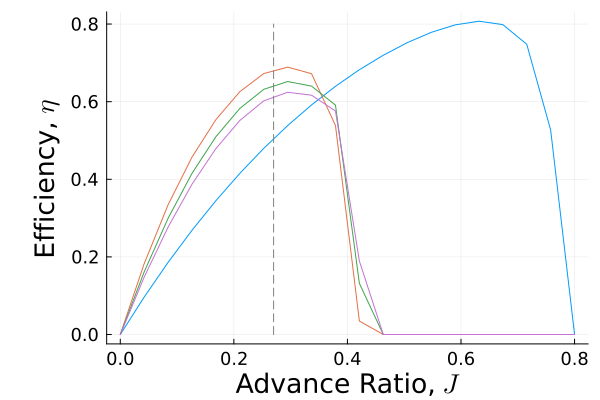
\includegraphics[width = .35\textwidth]{Plots/Figure_1.png}}
	\subfloat[]{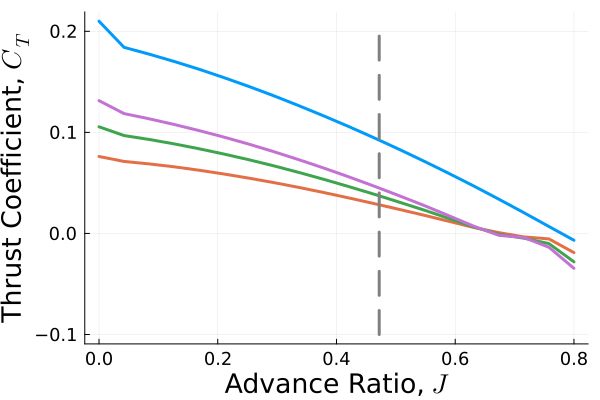
\includegraphics[width = .35\textwidth]{Plots/Figure_2.png}}

	\subfloat[]{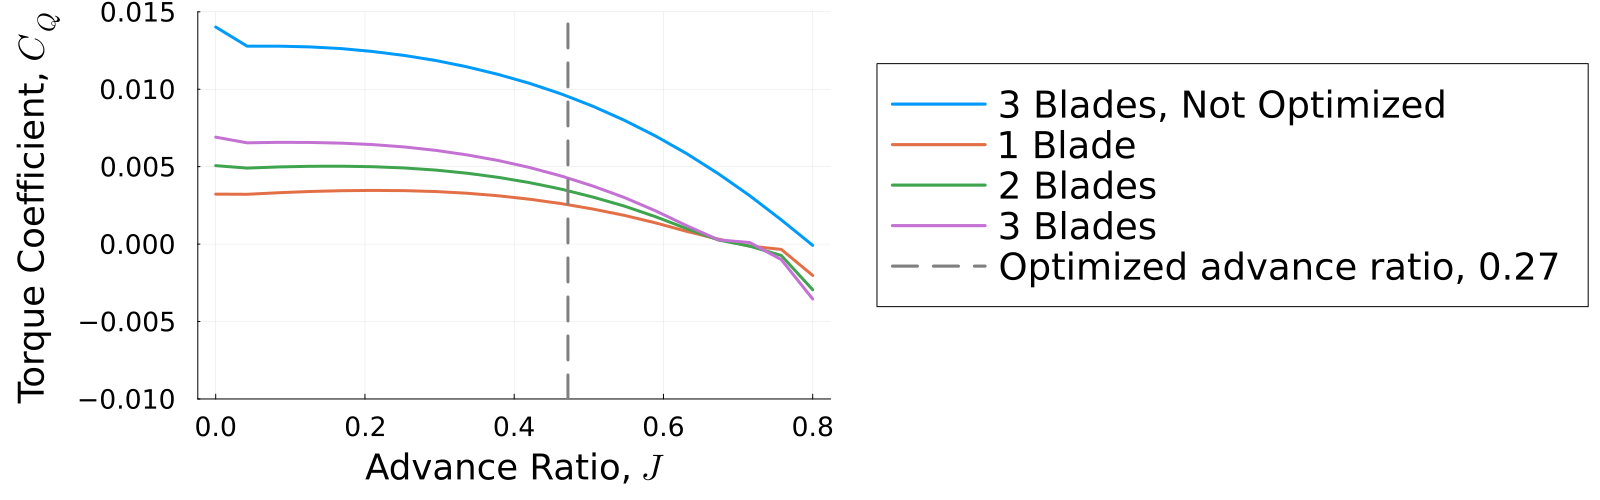
\includegraphics[width = .70\textwidth]{Plots/Figure_3.png}}\hspace{1em}
	\caption{Efficiency (a), thrust coefficient (b), and torque coefficient (c) compared at different advance ratios}
	\captionsetup{aboveskip=0pt,font=it}
	\label{efftqtab}
\end{figure}

If necessary, I could provide minimum thrust and torque coefficients as parameters along with the maximums shown below the objective function in equation \ref{optimization}. I could use these additional constraints to find the pitching angle and chord magnification that would provide the maximum efficiency while still maintaining some required thrust. The optimizer might not reduce the propeller to its minimum possible chord length in every case as it did in this optimization.

Table \ref{resultstab} shows the optimal pitching angles and chord magnifications found by SNOW.jl for each different propeller blade count. At the conditions listed in table \ref{ctab}, the optimal chord length magnification was constant, and the optimal twist angle was less than $-3^{\circ}$ for each propeller. These results prove a few things about the propeller designed.

\begin{table}[H]
 \centering
 \begin{tabular}{| c | c | c |} \hline
 	 \textbf{Blade count} & \textbf{chord length Multiplication} & \textbf{Pitching angle} \\ \hline
  	 3 (Default) & 1.0 & $0^{\circ}$ \\ \hline
  	 2 & 0.50 & $-2.70^{\circ}$ \\ \hline
  	 3 & 0.50 & $-2.88^{\circ}$ \\ \hline
  	 4 & 0.50 & $-2.94^{\circ}$ \\ \hline
 \end{tabular}
 \caption{Optimized chord magnification and pitching angles for different blade counts}
 \label{ctab}
\end{table}

First off, propellors with lower solidity appear to be more efficient. All of the propellors optimized had the lowest possible chord length allowed by the program used. Rotor solidity can be calculated with equation \ref{solid}. This shows that reducing the chord length, $c$, or the blade count, $n_{b}$, reduces the solidity, $\sigma$. The finding that lower solidity leads to greater efficiency seems reasonable, because wind turbine propellers, designed to efficiently harvest wind from the environment, have very low solidity according to this equation. This finding about propeller blades with less solidity being more efficient also agrees with Saraf, Nouli, Ravalet, and Bakir's findings.\cite{AxFlFan} 

\begin{equation}
	\begin{aligned}
	\sigma = \frac{c}{s} = \frac{c n_{b}}{2 \pi \sqrt{\frac{r_{h}^{2}+r_{t}^{2}}{2}}}
\end{aligned}
\label{solid}
\end{equation}

Table \ref{resultstab} shows that although the optimal pitching angles were very similar for all three different blade counts, they became minutely more negative as the blade count increased. This further decrease in the already negative pitching angle could be at least partially explained by the airfoil polars shown in figure \ref{afplot}. Increasing the pitching angle slightly above $-3^{\circ}$ would make its lift coefficient higher and its drag coefficient slightly lower. Figure \ref{afplot}, from airfoil analysis conducted earlier in the semester, shows that angles of attack near $-3^{\circ}$ for the NACA 4412 airfoil used in this design correspond to a very low drag coefficient and lower drag forces.

Changing the pitching angle of this propeller would change the forces and efficiency experienced by a propeller with a blade count of 2 differently than propellers with blade counts of 3 or 4, because the wake created by each propellor blade affects airflow over the blade next to it. This is why the curves in figure \ref{efftqtab} are shaped differently from each other, even though they are optimizations of propellors with the same airfoil and rotor profiles.

One problem with this optimization is that a propeller's efficiency is available as a function of the advance ratio, the thrust coefficient, and the power coefficient. The equation for efficiency is described by Andrew Ning in \emph{Computational Aerodynamics},\cite{ComAer} using the relations below, in equation \ref{etqeq}.

\begin{equation}
	\begin{aligned}
	\eta = J \frac{C_{T}}{C_{P}} \\
	\eta = \frac{T V_{\infty}}{T V_{\infty} + \frac{1}{2} \dot{m} (V_{w} - V_{\infty})^{2}}
	\end{aligned}
\label{etqeq}
\end{equation}

Ning also wrote that when thrust is increased for a propellor, it comes at the expense of decreased efficiency.\cite{ComAer} Conversely, a propellor optimization that maximizes efficiency will decrease its thrust coefficient. The torque and moments output by the optimized propellors did not even come near those of the original propellor. For example, the original propellor blades experienced a normal moment of $3.753 \times 10^{6}N \times m$, but the optimized propellor with the same blade count only experienced $3.808 \times 10^{5} N \times m$.

When I kept $J$ kept constant in this research, inspection of figure \ref{efftqtab} reveals that the optimizer maximized equation \ref{optimization} by minimizing $C_{P}$, which is equal to $C_{Q}$ multiplied by $2 \pi$. The torque coefficient $C_{Q}$ is significantly lower for each propeller. While the thrust coefficient $C_{T}$ did not decrease by as much as $C_{Q}$, it is still much lower than before. Although more efficient, the newly optimized propeller produces much less power and may be better suited for an entirely different environment than the one it started with.


\section{Conclusion}

In this optimization, I used Julia to find the 




















This optimization combined several different Julia packages to find the optimal angle of rotation and chord length for a propeller's efficiency. It found that propellers with very small chord lengths at negative angles of rotation were the most efficient. Other optimizations could be performed by simple editing of the code used in this research to find which propellers perform best in other applications or environments. 


\section{Acknowledgements}

The author thanks Adam Cardoza for mentoring him in learning the codes used in the FLOW Lab, directing his research, helping him through questions and challenges that he faced during his work.



\bibliography{Final_Report}

\end{document}
